\section{Nota teórica}
En esta sección se muestran las descripciones generales de todos los componentes usados para construir el circuito solicitado.
\subsection*{Microcontrolador ATTiny4313}
El ATtiny2313A/4313 es un microcontrolador CMOS de 8 bits de bajo consumo basado en el AVR mejorado.
Arquitectura RISC. Al ejecutar poderosas instrucciones en un solo ciclo de reloj, el ATtiny2313A/4313 logra rendimientos cercanos a 1 MIPS por MHz, lo que permite al sistema diseñador para optimizar el consumo de energía frente a la velocidad de procesamiento \cite{web}. Por lo que se requiere estudiar el diagrama de pines mostrado en la figura \ref{fig1}
\begin{figure}[H]
\centering
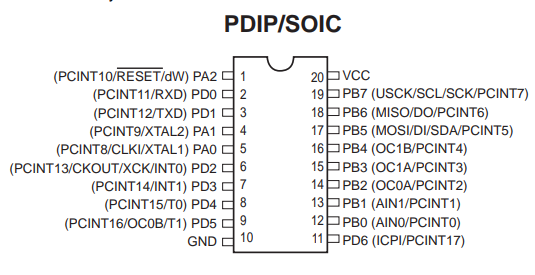
\includegraphics[width=.8\linewidth]{Imagenes/1.png}
 \caption{Pines del ATtiny4313. Tomado de \cite{web}.}
 \label{fig1}
\end{figure}
A continuación, se describen las características de cada pin para tener un mejor entendimiento de lo que se puede hacer con cada uno de ellos \cite{web}.
\begin{enumerate}
\item PA2-RESET/dW/PCINT10: RESET: entrada activa en bajo y activada por un 1 el \texttt{RSTDISBL} fuse. El pullup se activa y el controlador de salida y la entrada digital se desactivan cuando se usa el pin de RESET. \texttt{dW}: Cuando el fusible debugWIRE Enable (DWEN) está programado y los bits de bloqueo están sin programar, se activa el sistema debugWIRE dentro del dispositivo de destino. El pin RESET del puerto está configurado como un pin de I/O bidireccional de cable Y (drenaje abierto) con pull-up habilitado y se convierte en la puerta de enlace de comunicación entre el objetivo y el emulador. Sirve como I/O y tiene la opción de RESET. Solo que debe ponersele un 0 para que funcione como I/O. Tiene una resistencia interna de pull up. \texttt{PCINT10}: Fuente de interrupción de cambio de pin. El pin PA2 sirve como una fuente de interrupción externa.

\item PD0-RXD/PCINT11. \texttt{RXD}: UART receptor de datos. \texttt{PCINT11}: El pin PD0 sirve como fuente de interrupción externa.

\item PD1-TXD/PCINT12. \texttt{TXD}: UART transmisor de datos. \texttt{PCINT12}: El pin PD0 sirve como fuente de interrupción externa.

\item PA1-XTAL2/PCINT9. \texttt{XTAL2}: chip de reloj oscilador. Se utiliza como pin de reloj para todas las fuentes de reloj de chip excepto oscilador RC interno calibrable y reloj externo. Cuando se utiliza como pin de reloj, el pin no se puede utilizar como pin de I/O. Cuando se utiliza un oscilador RC interno calibrable o un reloj externo como en las fuentes de reloj del chip, PA1 sirve como un pin de I/O normal. Este pin sirve como fuente de interrupción externa.
\item PA0-\texttt{XTAL1/CLKI/PCINT8}. \texttt{XTAL1}: oscilador de reloj de chip. Se utiliza para todas las fuentes de reloj de chip excepto oscilador RC interno calibrable. Cuando se usa como pin de reloj, el pin no se puede usar como pin de I/O. Cuando se utiliza un oscilador RC interno calibrable como fuente de reloj de chip, PA0 sirve como pin de I/O. Este pin sirve como fuente de interrupción externa.
\item PD2-INT0/XCK/CKOUT/PCINT13. \texttt{INTO}: este pin sirve como fuente de interrupción externa para el MCU. \texttt{XCK}: USART Reloj de transferencia utilizado sólo en el modo de transferencia síncrona.\texttt{CKOUT}: reloj sistema de salida.
\item PD3-INT1/PCINT14. Ambas descripciones representan la misma equivalencia, ya que su objetivo final es que el pin PD3 sirve como fuente de interrupción externa.
\item PD4-TO/PCINT15. \texttt{TO}: timer/counter0 la entrada del reloj contador externo se habilita configurando (uno) los bits CS02 y CS01 en el registro de control del timer/counter0 (TCCR0).\texttt{PCINT15}: este pin sirve como fuente de interrupción externa.
\item PD5-OC0B/T1/PCINT16.\texttt{OC0B}:  Output Compare Match B. \texttt{T1}: La entrada del contador externo se habilita configurando (uno) los bits CS02
y CS01 en el registro de control del timer1/counter1 (TCCR1) \texttt{PCINT16}: este pin sirve como fuente de interrupción externa.
\item GND: nodo de tierra.
\item PD6-ICPI/PCINT17.\texttt{ICPI}: entrada de captura. Este pin puede actuar como un pin de captura de entrada para el timer/counter1. \texttt{PCINT17}: este pin sirve como fuente de interrupción externa.
\item PB0-AIN0/PCINT0. \texttt{AIN0}: es un comparador análogo de entrada positiva. Configure el pin del puerto como entrada con el pull-up interno apagado para evitar que la función del puerto digital interfiera con la función del comparador analógico \texttt{PCINT0}: este pin sirve como fuente de interrupción externa.
\item PB1-AIN1/PCINT1. \texttt{AIN1}: es un comparador análogo de entrada negativa. \texttt{PCINT1}: este pin sirve como fuente de interrupción externa.
\item PB2-OC0A/PCINT2.Output Compare Match A output. \texttt{OC0A}: el pin PB2 puede servir como salida externa para comparación de salida de timer/counter0 A. El pin debe configurarse como salida (configurando DDB2 igual 1) y cumplir esta función. \texttt{PCINT2}: este pin sirve como fuente de interrupción externa.
\item PB3-OC1A/PCINT3. \texttt{OC1A}:Output Compare Match A output. El pin PB3 puede servir como salida externa para comparación de salida de timer/counter1 A. El pin debe configurarse como salida (configurando DDB3 igual 1) y cumplir esta función. \texttt{PCINT3}: este pin sirve como fuente de interrupción externa.
\item PB4-OC1B/PCINT4. \texttt{OC1B}: Output Compare Match B output. Se puede configurar DDB4 igual a 1 para activar esta función. \texttt{PCINT4}: este pin sirve como fuente de interrupción externa.
\item PB5-DI/SDA/PCINT5.\texttt{DI}: Entrada de datos de interfaz serie universal en modo de tres cables. El modo de tres cables no anula las funciones normales del puerto, por lo que el pin debe configurarse como entrada.\texttt{SDA}: modo serial interfaz de datos de dos cables.\texttt{PCINT5}: este pin sirve como fuente de interrupción externa.
\item PB6-DO/PCINT6. \texttt{DO}: Salida de datos de interfaz serie universal en modo de tres cables. Modo de tres cables de salida de datos anula el valor de PORTB6 y se dirige al puerto cuando el bit de dirección de datos DDB6 es uno. Sin embargo, el bit PORTB6 aún controla el pull-up, lo que permite el pull-up si se ingresa la dirección y PORTB6 en 1. \texttt{PCINT6}: este pin sirve como fuente de interrupción externa.
\item PB7-USCK/SCL/PCINT7. \texttt{USCK}: interfaz serial de reloj modo de 3 cables. \texttt{SCL}: reloj serial para USI modo de dos cables. \texttt{PCINT7}: este pin sirve como fuente de interrupción externa.
\item VCC: fuente de alimentación.
\end{enumerate}

\subsubsection*{Características generales}
\subsection*{Lista de componentes}

\begin{table}[H]
\caption{Lista de equipos}
\label{table_2}
\begin{center}
\begin{tabular}{r|cc}
\hline
\textbf{Componente}&\textbf{Cantidad}&\textbf{Precio}\\
 \hline
- &-  &- \\  
-& - &- \\ \hline
 \textbf{Total}& &  \\
 \hline
\end{tabular}
\end{center}
\end{table}

\subsection*{Diseño del circuito}

\newpage